\chapter{Continuous Integration and Deployment}

\section*{Introduction}
This chapter delves into the core components that establish a robust CI/CD pipeline for our project. We'll explore the setup process, delve into the selection of a branching strategy, and dissect the configuration of pipelines designed for development, staging, and production environments. Each stage within these pipelines will be meticulously explained, highlighting its function and contribution to the overall workflow.
\section{Sprint backlog}
\begin{longtable}[c]{
    |p{.85\textwidth}|
    p{.11\textwidth}|
    }
    \caption{Sprint 2 backlog}
    \label{tab:Sprint2_backlog}                                                                            \\
    \hline
    research the different branching strategies and pick the appropriate one for this project & (2 points) \\
    \hline
    create the build pipeline and publish the artifacts for each environment                  & (3 points) \\
    \hline
    create the provisioning pipeline for the development environment                          & (3 points) \\
    \hline
    set up the management of the state file of the terraform in the pipeline                  & (2 points) \\
    \hline
    create the release pipelines for the staging and production environments                  & (3 points) \\
    \hline
    test the pipeline by pushing code to the different branches and checking the results      & (2 points) \\
    \hline
\end{longtable}
\section{Activities Completed}
\begin{itemize}
    \item \textbf{Azure DevOps account setup:} We created an Azure DevOps account to manage our CI/CD pipeline.
    \item \textbf{picking the right git branching strategy:} We chose the appropriate branching strategy to manage our codebase.
    \item \textbf{creation of the build pipeline:} We created a build pipeline that builds the dotnet core application and publishes the artifacts.
    \item \textbf{creation of the release pipelines:} We created the release pipelines that deploy the artifacts to the different environments depending on the branch.
    \item \textbf{testing the pipeline:} We tested the pipeline by pushing code to the different branches and checking the results.
\end{itemize}

\section{Version Control strategy}
\subsection*{ \textbullet\ The different branching strategies\cite{webArticle3}:}
\textbf{trunc based development:} In this strategy, requires no branches but instead, developers integrate their changes into a shared trunk at least once a day. This shared trunk should be ready for release anytime.
\begin{itemize}
    \item \textbf{Advantages:} Have better visibility over what changes other developers are making as commits are made directly into the trunk without the need for branches.
    \item \textbf{Desadvantages:} It can be difficult to monitor the quality of the codebase as there are no branches to isolate changes. This approach can be daunting for junior developers as they are interacting directly with the shared trunk.
\end{itemize}
\par
\textbf{github flow:} In this strategy, there is only one branch called the main branch. Developers create feature branches from the main branch, work on their features, and then create a pull request to merge their changes back into the main branch.
\begin{itemize}
    \item \textbf{Advantages:} This strategy is particularly suited for small teams and web applications and it is ideal when you need to maintain a single production version.
    \item \textbf{Desadvantages:} The lack of development branches makes this strategy more susceptible to bugs and so can lead to an unstable production code if branches are not properly tested before merging with the master-release preparation and bug fixes happen in this branch.
\end{itemize}
\par
\textbf{gitflow:} In this strategy, there are two main branches: the master branch and the develop branch. The master branch contains the production-ready code while the develop branch contains the latest code that is ready for release.
\begin{itemize}
    \item \textbf{Advantages:} Perhaps the most obvious benefit of this model is that it allows for parallel development to protect the production code so the main branch remains stable for release while developers work on separate branches.
    \item \textbf{Desadvantages:} Due to GitFlow's complexity, it could slow down the development process and release cycle. In that sense, GitFlow is not an efficient approach for teams wanting to implement continuous integration and continuous delivery.
\end{itemize}
\textbf{gitlab flow:} is a simpler alternative to GitFlow that combines feature-driven development and feature branching with issue tracking. GitLab Flow is great when you want to maintain multiple environments and when you prefer to have a staging environment separate from the production environment.
\begin{itemize}
    \item \textbf{Advantages:} It promotes teamwork and emphasizes code quality with a lean approach, encouraging practices like unit testing and CI/CD.
    \item \textbf{Desadvantages:} With more frequent integration, there's a higher chance of merge conflicts, especially in larger teams.
\end{itemize}
\begin{longtable}[c]{
    |p{.50\textwidth}
    |p{.10\textwidth}|
    p{.30\textwidth}|
    }
    \caption{the different situations where each branching strategy is suitable}
    \label{tab:gitStratagyTable}
    \\ \hline

    Product type and its release method                                                                                            & Team size & Applicable branching strategy                \\ \hline
    All                                                                                                                            & Small     & Trunk based development                      \\ \hline
    Products that support continuous deployment and release, such as SaaS products                                                 & Middle    & GitHub-Flow and TBD                          \\ \hline
    Products with a definite release window and a periodic version release cadence, such as iOS apps                               & Middle    & Git-Flow and GitLab-Flow with release branch \\ \hline
    Products that are demanding for product quality and support continuous deployment and release, such as basic platform products & Middle    & GitLab-Flow                                  \\ \hline
    Products that are demanding product quality and have a long maintenance cycle for released versions                            & Large     & Git-Flow                                     \\ \hline
\end{longtable}
\par
\textbf{Verdict:} Considering the table's comparison and the advantages and disadvantages listed, GitLab Flow emerges as the optimal choice for our project's workflow since we can leverage its strengths to establish a smooth, efficient, and quality-focused development process for our continuous deployment pipeline.
\subsection*{ \textbullet\ Description of the GitLab flow strategy:}
the GitLab flow strategy consists of 3 main branches: the main branch(develop), the staging branch(pre-prod), and the production branch(prod).

\begin{figure}[htbp]
    \centering
    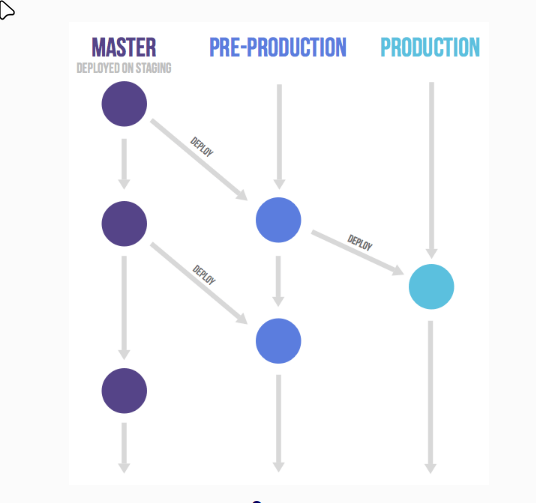
\includegraphics[width=0.6\textwidth]{gitLab.png}
    \caption{gitlab flow strategy}
    \label{fig:gitlab}
\end{figure}

\subsection*{ \textbullet\ Main branches:}
\begin{itemize}
    \item \textbf{the main branch(develop):} This branch is the default branch and contains the latest code that is ready for release. Developers create feature branches from the main branch, work on their features, and then create a pull request to merge their changes back into the main branch.
    \item \textbf{the staging branch(pre-prod):} This branch is used for testing the code by the QA team before it is deployed to the production environment. The staging branch is created from the main branch and is used to test the code in a production-like environment.
    \item \textbf{the production branch(prod):} This branch contains the production-ready code that is deployed to the production environment. The production branch is created from the staging branch and is used to deploy the code to the production environment.
\end{itemize}
\subsection*{ \textbullet\ Secondary branches:}
these branches are short-lived and are used to develop new features or fix bugs.
\begin{itemize}
    \item \textbf{feature branches:} These branches are created from the main branch and are used to develop new features. Once the feature is complete, a pull request is created to merge the changes back into the main branch.
    \item \textbf{Hotfix branches:} These branches are created from the production branch and are used to fix critical bugs in the production code. Once the bug is fixed, a pull request is created to merge the changes back into the production branch.
\end{itemize}

\section{The CI/CD pipelines}

\subsection*{ \textbullet\ The build pipeline:}
here's a detailed breakdown of the build pipeline for the .NET Core application:
\begin{itemize}
    \item \textbf{Fetch the code:} The pipeline starts by fetching the latest code from your GitHub repository or a pull request. This is done using a service connection that links our Azure DevOps account to the GitHub repository.
    \item \textbf{Build the code:} This stage involves two main tasks:
          \begin{itemize}
              \item \textbf{Restore dependencies:} The pipeline installs NuGet and restores the packages required for the project. Nuget is the package manager responsible for managing the various dependencies of this application.
              \item \textbf{Build the project:} The pipeline builds the .NET Core project using the dotnet build command.
          \end{itemize}
    \item \textbf{Run tests:} This stage involves running the unit tests and the integration tests to ensure the application functions as expected.
    \item \textbf{Publish artifacts:} The pipeline publishes the build artifacts to the Azure DevOps server. These artifacts are to be used by the release pipeline to deploy the application to the different environments.
\end{itemize}
\subsection*{ \textbullet\ The release pipeline:}
the release pipeline is the combination of the provisioning and deployment process. Here's a detailed breakdown of the different pipelines for the different environments:
\subsubsection*{ \textbullet\ The development environment:}
the dev environment is used for testing the code by the developers when a push request is made into the main branch and approval from another developer is required. it consists of the following stages:
\begin{itemize}
    \item \textbf{Fetch the artifacts:} The pipeline starts by fetching the latest artifact that contains the build of the application and the artifact that contains the terraform source code.
    \item \textbf{Deploy the infrastructure:} The pipeline deploys the infrastructure using the terraform source code using the service connection to the Azure subscription.
    \item \textbf{assign the variables:} The pipeline assigns the variables required for the deployment of the application like the name of the web app that is generated during deployment.
    \item \textbf{deploy the application:} The pipeline deploys the application to the web app using the artifact that contains the build of the application.
    \item \textbf{the approval stage:} After the pipeline notifies the responsible developer it waits for his approval to merge the code into the main branch after he is done reviewing the changes using the deployed application.
    \item \textbf{the destruction of the infrastructure:} This stage is used to destroy the infrastructure after the request has been approved or rejected.
\end{itemize}

\begin{figure}[htbp]
    \centering
    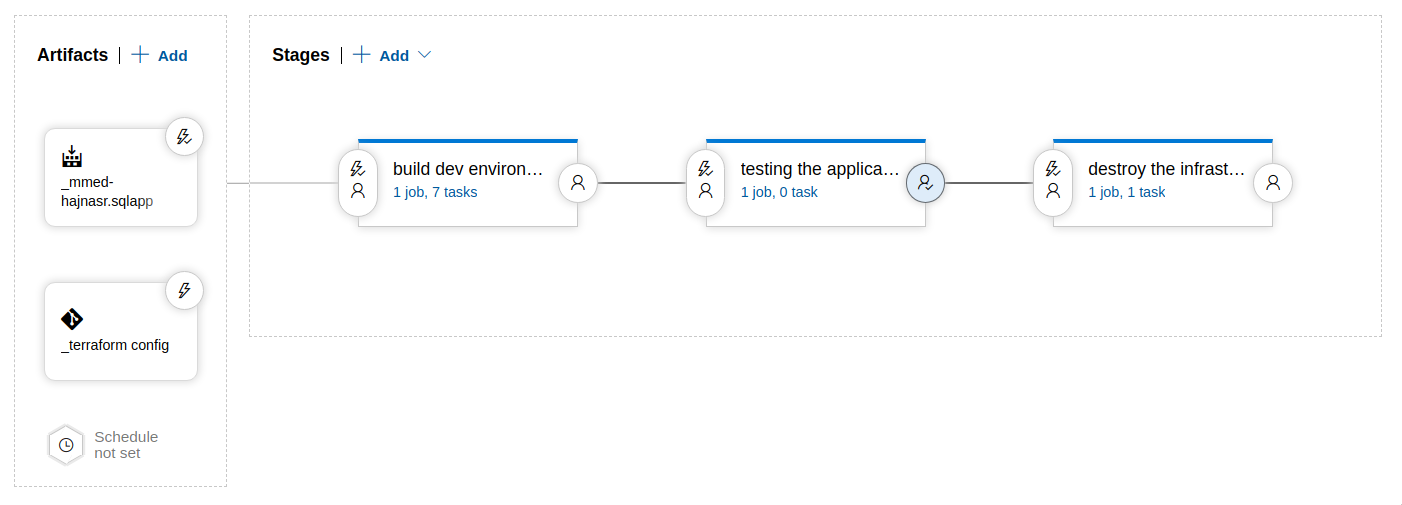
\includegraphics[width=0.9\textwidth]{dev_pipeline.png}
    \caption{development pipeline}
    \label{fig:devPipeline}
\end{figure}

\textbf{the benefits of this pipeline are:}
\begin{itemize}
    \item \textbf{fast feedback:} The pipeline provides fast feedback to the developers on the quality of the code.
    \item \textbf{cost savings:} The pipeline saves costs by destroying the infrastructure after the request has been approved or rejected. so that the infrastructure doesn't keep running when not needed.
    \item \textbf{multiple deployments:} The pipeline allows for multiple deployments in different infrastructures at once due to the randomly generated names. giving us the ability to test multiple pull requests at once.
\end{itemize}
\subsubsection*{ \textbullet\ The staging and the deployment pipelines:}
\noindent These pipelines share similar stages but differ in their triggers:
\begin{itemize}
    \item \textbf{Staging Pipeline:} Triggered by a push or merge to the pre-production (pre-prod) branch. This environment mirrors production as closely as possible for testing purposes.
    \item \textbf{Deployment Pipeline:} Triggered by a push or merge to the production (prod) branch. This pipeline deploys the application to the live environment used by end users.
\end{itemize}
\noindent The stages within these pipelines typically involve:
\begin{itemize}
    \item \textbf{Fetch the artifacts:} Similar to the development pipeline, this stage retrieves the latest Terraform configuration files and the recently built application artifact.
    \item \textbf{Deploy the infrastructure:} In the staging and production environments, the infrastructure is already deployed using the terraform files. so we directly deploy the application to the web app.
    \item \textbf{Notify Deployment Status:} Once the deployment is complete, the pipeline automatically notifies the designated manager (or team) about the success or failure of the process.
\end{itemize}
\textbf{the benefits of these pipelines are:}
\begin{itemize}
    \item \textbf{Increased Efficiency:} Automating deployments frees up valuable developer and operations time. They can focus on core activities like building new features, improving code quality, and resolving critical issues.
    \item \textbf{Reduced Risk of Errors:} Manual deployments are prone to human error. Staging and deployment pipelines automate the entire process, minimizing the chance of mistakes that could lead to application downtime or malfunctions.
    \item \textbf{Faster Release Cycles:} By automating the deployment process, teams can push new features and bug fixes to staging and production environments much quicker. This eliminates the time spent on manual tasks and allows for more frequent releases, keeping your software up-to-date and competitive.
\end{itemize}
\section{Challenges Faced}
\subsection*{ \textbullet\ Problem(Secure Terraform State Management in a Multi-Stage Pipeline):}
A critical hurdle encountered during CI/CD pipeline implementation was handling Terraform state files across stages. These files, generated during infrastructure deployment,  contain crucial details about the deployed infrastructure. Terraform relies on them to determine the current state for subsequent actions and this file was required by Terraform to destroy the infrastructure.
\par The initial solution involved saving the state file in an Azure storage account. However, this necessitated granting pipeline access to the storage, incurring potential costs.
\subsection*{ \textbullet\ Solution:}
Further exploration revealed a more efficient approach: utilizing the Azure CLI to destroy deployed resources. By relying solely on the readily accessible resource group name, the Azure CLI could effectively destroy resources after approval/rejection decisions, eliminating the need for storage access and associated costs.
\section*{Conclusion}
The meticulously crafted CI/CD pipeline significantly enhances the development process by automating deployments and infrastructure management. This automation not only minimizes manual work and the potential for errors but also facilitates faster deployments and cost savings through efficient infrastructure utilization.
Our selection of the GitLab Flow branching strategy fosters collaboration and ensures code quality throughout the development lifecycle.
\par
In conclusion, our new CI/CD pipeline empowers our team to deliver features and updates with remarkable efficiency while maintaining an unwavering commitment to quality. As we move forward, the next chapter will explore the various deployment strategies available and delve into the process of selecting and implementing the most suitable option for our specific project requirements.
